\chapter{Telegestore}
\label{capitolo5}
\thispagestyle{empty}
In questo capitolo analizzeremo la realizzazione di un software pensato per inviare dei comandi alle centrali e alle periferiche che permettono la telegestione. In particolare in questo capitolo ci concentreremo sul software che gestisce  la comunicazione tra la centrale operativa e le diverse centrali sia come comunicazione diretta sia tramite l'utilizzo di ricevitori.\\
Nel capitolo successivo, invece, concentreremo la nostra analisi sul modulo che permette all'operatore di inviare i comandi al software che analizzeremo in questo capitolo.\\
In particolare questo software comunicherà con le centrali della marca \emph{Tecnoalarm} che permettono una connessione diretta per la telegestione tramite l'ausilio di un protocollo proprietario, il \emph{TecnoOut}. Inoltre, come accennato nel capitolo precedente, sfrutteremo il ricevitore AteArgo per inviare dei comandi anche alle periferiche Webu All-In-One.\\
Per quanto riguarda le funzionalità di questo software il suo scopo principale è quello di inviare comandi alle diverse periferiche, tuttavia per fornire maggiori informazioni all'operatore, ogni qualvolta che viene avviata la telegestione si richiedono alle periferiche ed alle centrali lo stato delle zone e delle partizioni in modo da avere sempre sotto controllo la situazione corrente.\\
\section{I protocolli di comunicazione}
Analizziamo ora come questo software comunicherà con le centrali, in particolare non ci addentreremo molto nei protocolli in quanto essi sono proprietari, ma analizzeremo la struttura del pacchetto e la comunicazione con la centrale o con il ricevitore interessato. In particolare analizzeremo i pacchetti di controllo del protocollo AteArgo per l'invio di comandi tra questo software e il corrispettivo ricevitore, e il protocollo \emph{TecnoOut} per la comunicazione con le centrali Tecnoalarm.
\subsection{Protocollo TecnoOut}
Il protocollo TecnoOut è un protocollo proprietario di proprietà di TecnoAlarm studiato per la comunicazione tra le centrali e sistemi di gestione remota come software di domotica o, come nel nostro caso, sistemi di telegestione.
\subsubsection{La struttura del pacchetto}
Pur non potendo addentrarci in particolare nella struttura del pacchetto analizzeremo alcuni punti salienti. Questo protocollo è orientato al byte e più in particolare il paccetto ha una struttura molto semplice, esso è composto da:
$$
\begin{array}{c}
\langle STX\rangle\langle codice\rangle\langle comando\rangle\langle len\rangle\langle dati\rangle\langle CRC16\rangle\\
\end{array}	 
$$
I diversi campi sono rispettivamente:
\begin{description}
	\item[STX:] campo composto da un unico byte e che delimita l'inizio del pacchetto;
	\item[codice:] questo campo è composto da 3 byte e contiene il codice utente per permettere l'accesso alla centrale
	\item[comando:] campo composta da un unico byte che identifica il comando da eseguire sulla centrale;
	\item[len:] indica la lunghezza del campo dati, essa varia in base al tipo di operazione da eseguire sulla centrale;
	\item[dati:] questo campo contiene le informazioni aggiuntive da utilizzare insieme al campo \emph{comando};
	\item[CRC16:] questo è il campo di controllo errori che sfrutta un algoritmo di CRC a 16 bit calcolato sul resto del pacchetto. Questo campo ha una lunghezza di due byte.
\end{description}
\subsubsection{La criptazione del pacchetto}
Questo protocollo sfrutta la criptazione AES a 128 bit. Ogni attore della comunicazione deve conoscere una chiave denominata \emph{PassPhrase} la quale verrà utilizzata insieme al vettore di inizializzazione.\\
Durante la prima fase il client invia un vettore di 17 byte contenete nei primi 16 byte il vettore di inizializzazione e nel diciassettesimo un valore predefinito criptato con il vettore appena inviato e con la PassPhrase. Il server quando riceve questo pacchetto salva i primi 16 byte come vettore e decripta il diciassettesimo con tale vettore e con la PassPhrase se il diciassettesimo byte decriptato corrisponde con il valore predefinito allora l'inizializzazione si conclude con successo e tutti i pacchetti successivi saranno criptati con tale vettore. In caso contrario il client chiude la connessione e riprova.\\
Non ci soffermeremmo oltre sulla criptazione in quanto nel codice questa operazione sarà effettuata da una libreria esterna e non implementata direttamente.
\subsubsection{La connessione}
La connessione è una semplice connessione client server tramite protocollo TCP/IP nel quale il nostro software svolge la funzione di client e la centrale di allarme svolge quella di server. Questo significa che la centrale risponderà alle nostre richieste e non invierà messaggi se non interrogata. Durante la telegestione uno dei requisiti è quello di conoscere lo stato delle zone e delle partizioni perciò è necessario effettuare un polling per richiedere continuamente questi stati, ed all'inizio di ogni ciclo si controlla la presenza di nuovi comandi in coda.
In \fname{fig:contecno} vediamo come avviene la comunicazione, dopo la prima fase di inizializzazione del vettore di criptazione si prosegue con il ciclo di polling fino alla chiususra della connessione.
\begin{figure}
\centering
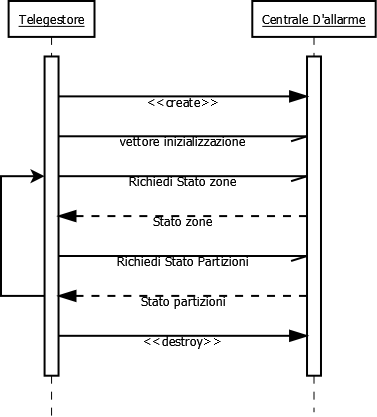
\includegraphics[width=0.7\linewidth]{pictures/contecno.png}
\caption{Scambio di messaggi tra software e centrali TecnoAlarm}\label{fig:contecno}	
\end{figure}
\subsubsection{I tipi di pacchetto}
In questo protocollo possiamo distinguere tre tipologie di pacchetto che sono:
\begin{itemize}
	\item messaggi di monitoring
	\item messaggi di pilotaggio
	\item messaggi di risposta
\end{itemize}
I messaggi di monitoring servono per richiedere alla centrale di fornire informazioni riguardo al suo stato e a quello delle sue zone, i messaggi di pilotaggio sono quelli inviati dal nostro software verso la centrale per farle eseguire delle operazioni, infine, i messaggi di risposta sono quelli inviati dalla centrale per rispondere alle nostre richieste.
\paragraph{Messaggi di monitoring}
I messaggi di monitoring sono quei messaggi che il nostro software dovrà inviare alla centrale per richiedere lo stato di alcuni elementi, in particolare a noi interessa richiedere lo stato dei seguenti elementi:
\begin{itemize}
	\item lo stato delle zone;
	\item lo stato delle partizioni;
	\item lo stato della centrale;
	\item lo stato dei programmatori orari.
\end{itemize}
Per stato delle zone noi intendiamo se il singolo sensore è escluso incluso oppure in allarme. Lo stato delle partizioni comporta sapere se esse sono inserite o disinserite o inserite solo in modo parziale. Per quanto riguarda le informazioni da conoscere sulla centrale, quelle che interessano a noi sono lo stato dell'alimentazione elettrica, quello della batteria e quello del tamper. Mentre l'unica informazione necessaria per i programmatori orari e se essi sono bloccati o in funzione.\\
Per reperire queste informazioni è necessario inviare alla centrale d'allarme il pacchetto formattato come precedentemente descritto con all'interno del campo codice un numero che ne identifica il comando. La centrale risponderà a questo comando inviando nel campo dati del pacchetto di risposta le informazioni. Prendendo come esempio le informazioni riguardanti la centrale noi inviamo il pacchetto specifico per richiedere queste informazioni e la centrale risponderà con un pacchetto con un unico byte nel campo dati. A questo byte deve essere applicata una maschera in AND per estrapolare le tre informazioni di cui necessitiamo.
\paragraph{Messaggi di pilotaggio}
I messaggi di pilotaggio servono per far eseguire delle azioni alla centrale d'allarme, per inviare i comandi da eseguire si utilizzano il pacchetto formattato così come indicato in precedenza con l'utilizzo di  opportuni codici. A differenza dei comandi di monitoraggio il campo dati questa volta contiene i valori da impostare sull'elemento selezionato. Ad esempio volendo escludo un opportuno sensore si invia alla centrale di allarme un pacchetto con l'opportuno valore nel campo comando e nei dati si inserisce il numero di zona e l'operazione da eseguire.\\
I comandi che interessano a noi sono solamente tre e riguardano le operazioni più comuni che gli operatori svolgono sulle centrali, ovvero, l'inclusione e l'esclusione di una zona, l'inserimento o il disinserimento di una partizione, ed infine il blocco o lo sblocco di un programmatore orario.
\paragraph{Messaggi di risposta}
I messaggi di risposta sono quelli che la centrale di allarme invia al nostro software essi possono essere di tre tipi:
\begin{itemize}
	\item ACK: in questo caso nel campo dati sono presenti eventuali risposte al messaggio inviato dal software come lo stato degli elementi richiesti.
	\item NACK: questo messaggio si riceve quando la centrale d'allarme non è in grado di interpretare il messaggio appena ricevuto e quindi non è in grado di dare una risposta.
	\item BUSY: questo tipo di messaggio di risposta si ottiene quando la centrale di allarme non è in grado di soddisfare le richieste perchè occupata a svolgere altre operazioni o a soddisfare richieste precedenti.
\end{itemize}
L'ultimo messaggio è da tenere molto in considerazione in quanto esso limita il tempo di polling per gli stati della centrale, il protocollo infatti specifica che le richieste devono essere inviate con un intervallo minimo di 500ms.
\subsection{Protocollo Urmet}
Questo protocollo è lo stesso del capitolo precedente, in questo caso però analizzeremo il pacchetto nel caso di ricezione degli stati degli ingressi e delle uscite e i pacchetti per impostare dei valori per le uscite.
\subsubsection{La struttura del pacchetto}
La struttura è quella che abbiamo visto nel capitolo precedente, si tratta di un protocollo basato su stringhe che formano una struttura XML con un tag di apertura seguito da una parte di header nella quali sono contenuti ora e data della trasmissione del pacchetto. Nel corpo del pacchetto invece troviamo le informazioni vere e proprie che dipendono dal tipo di pacchetto.
\subsubsection{La connessione}
Come si è visto la connessione con il software AteArgo è una connessione di tipo locale client-server nel quale il software di Urmet ricopre il ruolo di server. Tuttavia, pur essendo esso un server non permette la connessione di molteplici client questo ha comportato una problematica in quanto la connessione è necessaria al software ricevitore per mantenere la ricezione degli allarmi. Questo ci ha obbligati a pensare ad un meccanismo veloce e sicuro per far si che il ricevitore potesse inviare i comandi generati dal telegestore. Il meccanismo adottato è stato quello di una connessione socket tra Ricevitore e Telegestore, il telegestore invia una stringa ad un server che viene eseguito ogni volta che viene avviato il software di Ricezione. Questo meccanismo permette una comunicazione più rapida di quella che si avrebbe inserendo il comando in una tabella del database. 
Inoltre, questo tipo di comunicazione è stata pensata con un meccanismo di \emph{Reques-Replay} ed è quindi piuttosto affidabile.\\
Come nel caso precedente si attua un meccanismo di polling per richiedere lo stato degli ingressi e delle uscite di una determinata centrale, tuttavia in questo caso il polling no può essere molto stringente in quanto il software AteArgo effettua ogni volta la connessione con la centrale e non la mantiene aperta.
\subsubsection{I tipi di pacchetto}
Come abbiamo detto i tipi di pacchetto necessari per permettere di implementare le funzionalità richieste sono tre:
\begin{itemize}
	\item Pacchetto di richiesta degli stati
	\item Pacchetto di comunicazione degli stati
	\item Pacchetto di comando
\end{itemize}
\paragraph{Pacchetti di richiesta}
In questo tipo di pacchetto abbiamo che l'attributo del campo body è di tipo \emph{INO} nel campo body è presente solo l'identificativo della periferica di cui si vogliono conoscere gli stati.
\paragraph{Pacchetti di comunicazione degli stati}
In questo tipo di pacchetto abbiamo che l'attributo del campo body è uguale a quello della richiesta degli stati. In questo campo dopo le normali informazioni per identificare la periferica si ha una serie di campi per ogni ingresso uscita che ne stabiliscono se è un contatto d'ingresso oppure un contatto d'uscita, se esso è impostato in modalità \emph{''normalmente aperto''} oppure in modalità \emph{''normalmente chiuso''} ed infine lo stato del contatto.
\paragraph{Pacchetto di comando}
In questo caso il pacchetto di comando contiene nella parte body le informazioni per identificare la centrale su cui effettuare i comandi e i conttati da attivare o disattivare.
\subsection{Protocollo Telegestore-Ricevitore}
Come abbiamo visto nella paragrafo precedente per permettere una comunicazione veloce ed efficente tra il telegestore e il ricevitore che invia i comandi si è deciso di instaurare una connessione socket di tipo request-reply tra i due software.\\
I due software si scambiano dei messaggi basati sullo stesso protocollo interno pensato per la comunicazione tra il server JBoss e il software di telegestione che vedremo nel capitolo successivo. Tuttavia qui accenniamo ad alcuni aspetti di questo pseudo-protocollo.\\
I pacchetti non sono altro che stringhe contenenti diversi campi separati da un carattere \emph{'';''}. I messaggi scambiati tra il telegestore e il software di ricezione hanno il seguente formato:
\begin{center}
	\textit{ce\_id;COM;tipo;numero;comando}
\end{center}
dove \emph{ce\_id} è il codice che identifica la centrale, \emph{tipo} indica su quale elemento eseguire il comando se esso è una zona o una partizione. Il campo \emph{numero} indica il numero dell'elemento sul quale eseguire e, infine, il campo \emph{comando} contiene un codice per indicare quale azione sull'elemento identificato. Mentre il ricevitore, una volta eseguito il comando rimanda il pacchetto con indietro con l'aggiunta di un campo dopo comando con \emph{OK} se il comando è andato a buon fine o con \emph{KO} se il comando è fallito.
\subsection{Altri protocolli}
Mentre scriviamo sono in implementazione nuovi protocolli di telegestione, alcuni simili o comunque riconducibili a quelli già analizzati come il \emph{CEI-ABI} protocollo standard per la ricezione di allarmi e la gestione di centrali d'allarme. La particolarità di questo protocollo è che mantiene sempre aperta la connessione con la centrale. Questa particolarità comporta un meccanismo tipo quello adottato con urmet per inviare i comandi in quanto è possibile aprire un'unica connessione ed è necessaria per la ricezione degli eventi.\\
Una seconda tipologia di telegestione in fase di sviluppo invece si basa sull'invio alle centrali di SMS preformattati e la centrale d'allarme risponde contattando la centrale operativa ed inviando le informazione richieste tramite i normali canali di comunicazione. Per questo tipo di comunicazione non è prevista la verifica dell'invio del comando e la comunicazione avviene tramite dei modem GPRS collegati su porte seriali.
\section{La struttura dati}